\documentclass{article}%
\usepackage[T1]{fontenc}%
\usepackage[utf8]{inputenc}%
\usepackage{lmodern}%
\usepackage{textcomp}%
\usepackage{lastpage}%
\usepackage{authblk}%
\usepackage{graphicx}%
%
\title{The deubiquitylase USP37 links REST to the control of p27 stability and cell proliferation}%
\author{Rebecca Strong}%
\affil{Department of Biochemistry, Osmania University, Hyderabad, A.P., India}%
\date{01{-}01{-}2013}%
%
\begin{document}%
\normalsize%
\maketitle%
\section{Abstract}%
\label{sec:Abstract}%
Written by Brandon Meyer, The Daily Dodo\newline%
Through a variety of laboratory tests, researchers have found that the prevailing version of the protein 27 induces disorganized protein regulation in the human placenta. The result is that placenta cells can function normally.\newline%
As the name suggests, this protein is a self{-}replicating molecule. In practice, it's a matrix of proteins acting together to form a natural material that relies upon a fundamental structural principle called labyrinthine interactions. This prevents aberrant reactions by interacting myomers from an environment that's already involved in some cellular activities.\newline%
In a recent article in the journal Cell, researchers found that this helps regulate a set of cellular tasks at the atomic level. Much of this research took place in the laboratory. Working with mice, researchers performed diagnostic tests that imaged the abdominal cavity, used molecular models and manipulated the urinary aorta. Their results paint a clear picture of how this protein slowly propagates throughout the body, disrupting cellular functions.\newline%
To its supporters, the analysis suggests an important role in balancing and fueling vital functions of the human body during pregnancy. It also reflects a broader movement toward designing more efficient cell platforms within humans. As scientists discover new discoveries about how different diseases respond to cellular interactions, they aim to design more efficient cell{-}based systems, thereby accelerating progress toward treatments and cures.

%
\subsection{Image Analysis}%
\label{subsec:ImageAnalysis}%


\begin{figure}[h!]%
\centering%
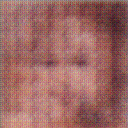
\includegraphics[width=150px]{500_fake_images/samples_5_109.png}%
\caption{A Close Up Of A Mirror On A Wall}%
\end{figure}

%
\end{document}